\chapter{Background}\label{chapter:background}

One of the major prerequisites for conducting calculations on tangrams as well as individual puzzle pieces is a representation that supports the efficient computation of different properties of both individual and multiple pieces. The calculations involved in this project include, among others, the transformation of pieces, the detection of overlap between pieces and determining if a shape is completely covered by the seven tans. This chapter describes the required geometrical primitives and additionally shows how restricting the possible rotations of a tan to multiples of $45^{\circ}$ leads to some simplifications.

\section{Tangram and Tans}

The puzzle pieces as well as tangram patters are polygons, which are usually represented by a sequence of points or line segments. As the puzzle pieces in tangram are always the same, this representation can however be simplified. When a tan is positioned on a two-dimensional plane it can already be fully described by its type, its position. There are five different tan types: the three-sided pieces: large, medium and small triangles, of which two large and two small triangles exist, and the four-sided pieces: square and parallelogram. In contrast to the other shapes, the parallelogram does not exhibit reflection symmetry in the same manner as the other pieces, but is rotationally symmetric. Therefore, it is the only piece that may have to be flipped in order to solve a tangram. The position of a tan can be defined by the position of just one vertex and the orientation of the tan, leading to a more lightweight representation of tans that can be easily updated in case the tan is transformed. 

A tangram can then be simply described by its tans. The outline of a shape is useful for displaying tangrams as well as correctly detecting alternative solutions to an originally generated one. Additionally the outline plays an important role in the definition of interestingness measures. As the randomly generated tangrams are supposed to be connected, the outline of a tangram is a potentially self-touching polygon that also possibly contains holes.

All things considered, the required components for representing tans and tangrams are points defined by two coordinates in a two-dimensional plane and line segments and thus these will be studied more closely in the following.

\section{Coordinates}

Taking a look at the way the tan pieces are constructed from cutting a square, one can see that the irrational number $\sqrt{2} \approx 1.4142135623$ is essential for calculations surrounding tans. Figure \ref{figure:dim} shows the dimensions of the tan pieces when the side length of the square is set to 4. With this setting, the hypotenuses of the two large triangles have length 4 and their legs have length $2\sqrt{2}$. The figure also shows that each tan is composed of a number of base triangles like the one displayed to the right of the square. 

\begin{figure}[h!]
\centering
\begin{tikzpicture}
\draw[help lines] (0,0) grid (4,4);
\fill [Color2, opacity = 0.5] (0,0)--(4,0)--(2,2)--(0,0);
\fill [ Color1, opacity = 0.5] (4,0)--(4,4)--(2,2)--(4,0);
\fill [ Color5, opacity = 0.5] (4,4)--(3,3)--(1,3)--(2,4)--(4,4);
\fill [ Color3, opacity = 0.5] (2,4) -- (0,4) -- (0,2) -- (2,4);
\fill [ Color7, opacity = 0.5] (1,3)--(3,3)--(2,2)--(1,3);
\fill [ Color4, opacity = 0.5] (1,3) -- (2,2) -- (1,1) -- (0,2) -- (1,3);
\fill [Color6, opacity = 0.5] (0,0) -- (1,1) -- (0,2) -- (0,0);
\draw (0,0) -- (4,0);
\draw (0,1) -- (4,1);
\draw (0,2) -- (4,2);
\draw (0,3) -- (4,3);
\draw (0,4) -- (4,4);
\draw (0,0) -- (0,4);
\draw (1,0) -- (1,4);
\draw (2,0) -- (2,4);
\draw (3,0) -- (3,4);
\draw (4,0) -- (4,4);
\draw (5,1) -- (6,1); 
\draw (5.5, 0.7) node{1};
\draw (4.8, 1.5) node{1};
\draw (5.65, 1.8) node{$\sqrt{2}$};
\draw (5,1) -- (5,2);
\draw (6,1) -- (5,2);
\end{tikzpicture}
\caption{Dimensions of the tans}
\label{figure:dim}
\end{figure}
$\sqrt{2}$ will therefore occur in many coordinates of points and direction vectors and would implicate a heavy use of floating point arithmetic if coordinates would work with the number directly. Floating point arithmetic is computationally more expensive than integer arithmetic and requires special care in comparison operations due to rounding errors. A solution to this problem is basing all calculations on the commutative ring 
\[\mathbb{Z}[\sqrt{2}] = \{ a + b \sqrt{2} \;|  \; a,b \in \mathbb{Z}  \}\]
which essentially means that each number within a coordinate is represented by two integers. 
The fact that $\mathbb{Z}[\sqrt{2}]$ is closed under addition and multiplication. All other requirements for commutative rings can be shown in a similar way or be directly derived from knowledge about $\mathbb{Z}$.
\begin{align*}
(a + b \sqrt{2}) + (c + d \sqrt{2}) &= (a+c) + (b+d) \sqrt{2}\\
(a + b \sqrt{2}) * (c + d \sqrt{2}) &= (ac + bd*\sqrt{2}*\sqrt{2}) + (ad\sqrt{2} + bc\sqrt{2}) \\&= (ac + 2bd) + (ad+bc)\sqrt{2}
\end{align*}

The usage of $ \mathbb{Z}$ as the basis for coordinates is only possible due to the dimensions of the tans and the fact that tangrams have to be connected and none of the tans can overlap. Additionally, rotations by $45^\circ$ fit nicely into this scheme as $\sin(45^{\circ}) = \cos(45^{\circ})=  \frac{1}{2}\sqrt{2}$ and direction vectors within tans have only horizontal or vertical direction or take a form where both coordinates contain odd integers. This means that the factor of $\frac{1}{2}$ does not cause any problems. 
\section{Points}

Points are represented by x- and y-coordinates that take the form of the coordinates described in the previous sections. At some points during the computation an extended representation is advantageous, particularly when points are being transformed, i.e. rotated or translated. Before a transformation, a point is transferred into projective plane, which is basically an euclidean plane embedded in the three dimensional space, here at $z = 1$. This, together with a projective definition of lines, leads to very interesting principles for intersecting lines and connecting points, but more importantly has a great impact on how the transformation of points can be calculated. The representation of a transformation within the usual euclidean space depends on the type of transformation. The description of a translation is different from the one of a rotation. Therefore, the composition of multiple transformations results in complicated expressions. This is not the case for the projective plane. Its properties lead to the uniform representation of transformations as matrices and thus simplifies the composition of arbitrary transformations to simple matrix multiplication. Table \ref{transformation} shows how different transformations of a point $(x, y)^{T}$ in the euclidean and the projective plane can be expressed \cite{richter11}.
\begin{table}[htbp]
  \centering
\begin{tabular}{@{}lcc@{}}
\toprule
\textbf{Transformation} & \textbf{Euclidean Plane} & \textbf{Projective Plane} \\
\midrule 
\addlinespace[6.2pt]
 Rotation & $
%\begin{pmatrix} x\\ y \end{pmatrix} \mapsto 
\begin{pmatrix}
 \cos(\alpha) & -\sin(\alpha)\\
 \sin(\alpha) & \cos(\alpha) 
\end{pmatrix} \begin{pmatrix} x\\ y \end{pmatrix}$ & $
%\begin{pmatrix} x\\ y \\ 1 \end{pmatrix} \mapsto 
\begin{pmatrix}
 \cos(\alpha) & -\sin(\alpha) & 0 \\
 \sin(\alpha) & \cos(\alpha) & 0\\
 0 & 0 & 1 
\end{pmatrix} \begin{pmatrix} x\\ y \\ 1 \end{pmatrix}$ \\ \addlinespace[6.2pt]
 Translation & $
%\begin{pmatrix} x\\ y \end{pmatrix} \mapsto 
\begin{pmatrix}
 x\\
 y\end{pmatrix} + \begin{pmatrix}
 t_x\\
 t_y \end{pmatrix}$ & $
%\begin{pmatrix} x\\ y \\ 1 \end{pmatrix} \mapsto
 \begin{pmatrix}
 1 & 0 & t_x \\
 0 & 1 & t_y\\
 0 & 0 & 1 
\end{pmatrix} \begin{pmatrix} x\\ y \\ 1 \end{pmatrix}$ \\ \addlinespace[6.2pt]
 \bottomrule
\end{tabular}%
  \caption{Comparison of transformations in euclidean and projective plane}
  \label{transformation}%
\end{table}%

Aside from the transformation of an individual point and the obvious combination of points to form direction vectors, there exist some calculations to derive information about multiple points. The determinant of the $2 \times 2$ matrix containing two direction vectors as columns is one example. It helps to calculate the relative orientation between three points. Given three points $A,B$ and $C$ the determinant containing $(C-A)$ and $(C-B)$ determines in which order the points are positioned or whether $C$ is on the right or left side of segment $AB$. $A,B$ and $C$ are collinear if the determinant is zero. For values smaller than zero the triangle formed by the three points has been defined in a counter-clock order, for values larger than zero the points are given in clockwise order (see Figure \ref{relative}).

\begin{figure}[h!]
\centering
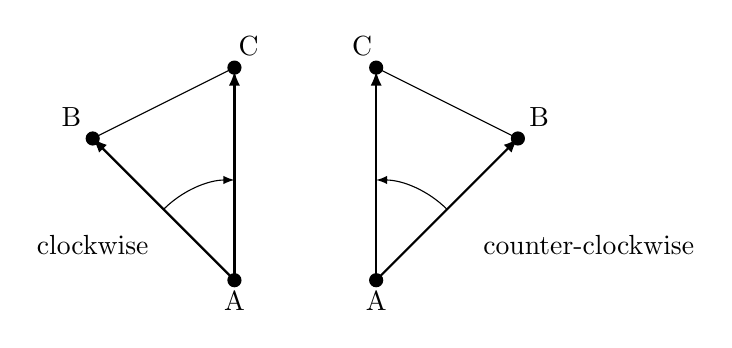
\begin{tikzpicture}[scale=0.9]
\draw[thick, -latex] (2, 0) -- (0,2);
\draw[thick, -latex] (2, 0) -- (2,2.95);
\draw (0,2) -- (2,3);
\fill[black] (2,0) circle (0.1);
\fill[black] (0,2) circle (0.1);
\fill[black] (2,3) circle (0.1);
\draw[-latex] (1,1) arc (135:90:1.4142);
\draw (2,-0.3) node{A};
\draw ((-0.3,2.3) node{B};
\draw (2.2,3.3) node{C};
\draw(0, 0.5) node{clockwise};
\draw[thick, -latex] (4, 0) -- (6,2);
\draw[thick, -latex] (4, 0) -- (4,2.95);
\draw (6,2) -- (4,3);
\fill[black] (4,0) circle (0.1);
\fill[black] (6,2) circle (0.1);
\fill[black] (4,3) circle (0.1);
\draw[-latex] (5,1) arc (45:90:1.4142);
\draw (4,-0.3) node{A};
\draw (3.8,3.3) node{C};
\draw(6.3,2.3) node{B};
\draw(7, 0.5) node{counter-clockwise};
\end{tikzpicture}
\caption{Relative orientation of three points or turning direction of consecutive line segments}
\label{relative}
\end{figure}
The concept of relative orientation of three points is applied in multiple algorithms throughout this project. Two examples are a point-in-polygon algorithm that determines whether a given point is inside, outside or on the outline of a polygon and the computation of the convex hull of a shape or a set of points. One possibility to determine if a point lies inside a polygon is calculating the winding number which characterizes the number of times a polygon winds around a point \cite{hormann01}. The winding number is computed by casting a horizontal ray from the given point to right and then increasing and decreasing the winding number depending on whether a crossed line segment where the points are sorted according to their x-coordinate, points downwards or upwards.

The convex hull of a shape can be computed using a technique called Graham's scan \cite[Chapter~33]{cormen09}. It relies on first sorting all points according to their angle in respect to the most lower left point and filtering out all points that have the same angle as a point further away form the most lower left point. Then, the sorted points are traversed and added or removed from the hull depending on their relative orientation to the two previously added points. This algorithm inspired the outline computation that will presented in Section \ref{outline}.
\section{Line Segments}

\begin{figure}[h!]
\centering
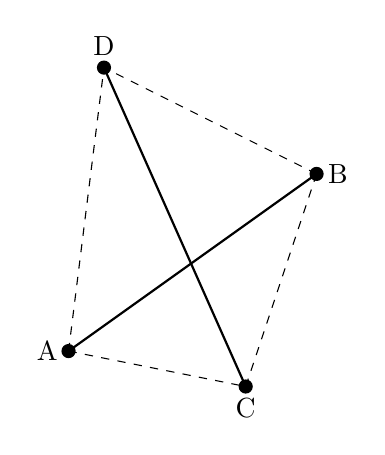
\begin{tikzpicture}[scale=0.9]
\draw[thick, circle] (0, 0.5) -- (3.5,3);
\draw[thick, circle] (2.5, 0) -- (0.5,4.5);
\fill[black] (0, 0.5) circle (0.1);
\fill[black] (3.5,3) circle (0.1);
\fill[black] ((2.5, 0) circle (0.1);
\fill[black] (0.5,4.5) circle (0.1);
\draw[dashed] (0, 0.5) -- (0.5,4.5);
\draw[dashed] (0, 0.5) -- (2.5, 0);
\draw[dashed] (2.5, 0) -- (3.5,3);
\draw[dashed] (3.5,3) -- (0.5,4.5);
\draw (-0.3,0.5) node{A};
\draw (3.8,3) node{B};
\draw(2.5, -0.3) node{C};
\draw (0.5,4.8) node{D};
\end{tikzpicture}
\caption{Intersecting line segments}
\label{segments}
\end{figure}
Line segments are defined by their two endpoints. For some algorithms it makes sense to sort the points such that the first point of a segment is always the one with smaller x-coordinate or smaller y-coordinate if the x-coordinates are equal. The two questions that arise in the context of line segments are whether two line segments intersect or if a line segment contains a point. Both can be addressed by applying the concept of relative orientation of three points, introduced before. As seen in Figure \ref{segments}, two line segments intersect if the points of one line segment lie on opposite sides of the other line segment and vice versa. \cite[Chapter~33]{cormen09}. When determining wether a point $P$ lies on a line segments $AB$, a determinant of 0 for $(B-A)$ and $(P-A)$ shows that the three points are collinear. If this is the case, the the parameter $t$ for which $P = A + t*(B-A)$ holds, can be calculated. If $t$ is between 0 and 1, the point lies on the segment, as $A + t*(B-A)$ defines the line through $A$ and $B$.
